\chapter{器官发生：四足动物肢的构建}\label{ch:b2:limb-organogenesis}

鸡蛋产出三天后，胚胎两侧体壁上各出现一个
针头大小的隆起。再过四天，它已成为翅膀，
具有肱骨、桡骨与尺骨、腕部和三根指，
顺序正确，长度合适，肌肉附着于正确的骨骼上。
切去隆起边缘增厚的皮肤，翅膀便停止生长；
将其后缘的一小片组织移植到前缘，
它便长出镜像对称的六根指。\omterm{def:b2:limb-organogenesis:bud}{肢芽}是
\emph{器官发生}的经典案例——即由一片细胞
借助信号构建器官，这些信号告诉每个细胞
在远近、前后与背腹方向上所处的位置——解码这一过程的实验
堪称生物学中最清晰的一批。本章追踪\omterm{def:b2:limb-organogenesis:bud}{肢芽}
从向外生长到形成骨骼的全过程。

\section{肢芽及其三条轴}

\begin{definition}[肢芽]\label{def:b2:limb-organogenesis:bud}
\index{肢芽}\index{顶端外胚层嵴}\index{极性活性区}
\emph{肢芽}是\emph{侧板中胚层}的隆起，
外被外胚层覆盖，发生于体侧的一个固定位置
（即\emph{肢区}）处，此处体轴的 Hox 编码允许其发生；
芽体的中胚层将形成骨、软骨、肌腱和真皮，
由\omterm{prop:b2:vertebrate-development:neurulation}{体节}迁入的细胞将形成肌肉。
芽体具有三条轴，各由一个信号中心调控。
\emph{近–远轴}（从肩到指尖）：\emph{顶端
外胚层嵴}（AER）：沿顶端的增厚外胚层条带，
分泌\omterm{prop:b2:limb-organogenesis:aer}{成纤维细胞生长因子}（FGFs），使其下方的
中胚层保持分裂而未分化。
\emph{前–后轴}（从拇指到小指）：\emph{极性活性区
}（ZPA）：位于后缘的一块中胚层，
分泌\omterm{thm:b2:vertebrate-development:gradient}{形态发生素}\emph{Sonic hedgehog}（Shh）。
\emph{背–腹轴}（从手背到手掌）：背侧
外胚层分泌 Wnt7a。前肢芽与后肢芽外形相似，并
使用相同的信号；二者的区别在于一个转录因子，
其在芽体出现之前即已表达（前肢为 Tbx5，
后肢为 Tbx4），这便是翅膀成为翅膀的缘由。
\end{definition}

\begin{omfigure}
\begin{tikzpicture}[every node/.style={font=\scriptsize}, >=stealth]
  % flank
  \fill[omExo!25] (0,-2.2) rectangle (1.2,2.2); \node[rotate=90] at (0.6,0) {体壁（体侧）};
  % bud outline: paddle
  \draw[thick, fill=omDef!10] (1.2,1.4) .. controls (3.0,1.9) and (5.2,1.6) .. (5.8,0.3) .. controls (5.9,-0.3) and (5.2,-1.6) .. (3.4,-1.7) .. controls (2.4,-1.8) and (1.6,-1.5) .. (1.2,-1.4);
  % AER along the tip
  \draw[line width=3pt, omThm] (5.2,1.3) .. controls (5.9,0.6) and (5.9,-0.6) .. (5.0,-1.4);
  \node[omThm, anchor=west, align=left] at (6.1,0.9) {顶端外胚层嵴（AER）：\\FGFs，近–远轴向生长};
  % ZPA posterior
  \draw[thick, omProp, fill=omProp!50] (2.4,-1.1) ellipse (0.55 and 0.4);
  \draw[omProp] (2.4,-1.5) -- (2.4,-2.0);
  \node[omProp, anchor=north, align=center] at (2.6,-2.0) {ZPA（后缘）：\\Sonic hedgehog，前–后轴};
  % dorsal ectoderm
  \draw[line width=2pt, omDef!70!black] (1.4,1.55) .. controls (3.0,2.0) and (5.0,1.7) .. (5.4,1.2);
  \node[omDef!70!black, anchor=south] at (3.4,2.05) {背侧外胚层：Wnt7a，背–腹轴};
  % axes
  \draw[->, thick] (1.5,-3.1) -- (5.5,-3.1); \node[below] at (3.5,-3.15) {近端 $\to$ 远端};
  \draw[->, thick] (10.6,-1.6) -- (10.6,1.2); \node[right, align=left] at (10.7,-0.2) {后 $\to$ 前 \\（从小指到拇指）};
\end{tikzpicture}

{\small 从上方观察的鸡胚\omterm{def:b2:limb-organogenesis:bud}{肢芽}及其三个信号中心：沿顶端的
AER 驱动生长，后缘的 ZPA 决定各指的排列，背侧
外胚层区分手背与
手掌。}
\end{omfigure}

\begin{omfigure}
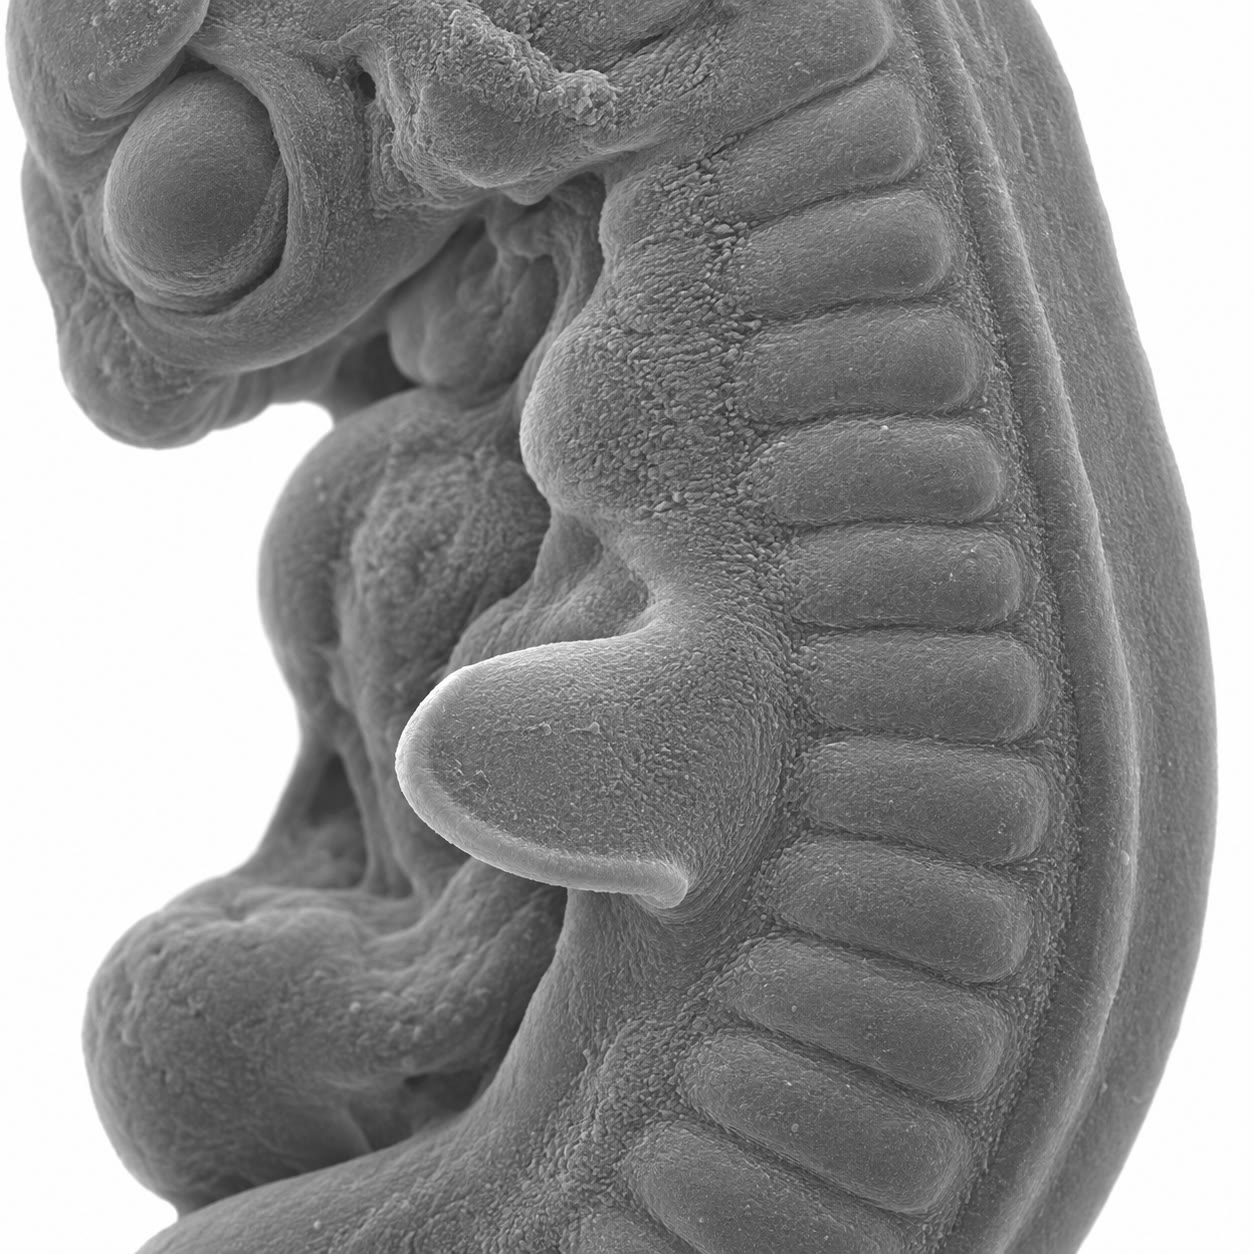
\includegraphics[width=0.42\linewidth]{images/book4/ai/b4-11-limb-bud.jpg}

{\small 扫描电子显微镜下的鸡胚：
沿躯干排列的一列\omterm{prop:b2:vertebrate-development:neurulation}{体节}，以及体侧的桨状
\omterm{def:b2:limb-organogenesis:bud}{肢芽}，其边缘有增厚的嵴。}
\end{omfigure}

\section{生长：近–远轴}

\begin{proposition}[顶端外胚层嵴]\label{prop:b2:limb-organogenesis:aer}
\index{成纤维细胞生长因子}\index{进展区}
AER 对生长不可或缺，其 FGFs 亦足以
使其下方的中胚层（即\emph{\omterm{prop:b2:limb-organogenesis:aer}{进展区}}）约每十二
小时分裂一次，随顶端推进而离开该区的细胞
停止分裂、凝结并分化。骨骼以
近–远轴顺序形成——\emph{柱节}（肱骨或股骨）、
\emph{轭节}（桡骨与尺骨，胫骨与腓骨）、\emph{自节}
（腕部与指）——各段在芽体生长过程中依次确定，
而各段对应于嵌套的 Hox 基因表达域，
（Hoxa/d 9--10 位于柱节，11 位于轭节，13 位于
自节）。\omterm{def:b2:limb-organogenesis:bud}{肢芽}在四天内长度增长约十倍，
而嵴信号的作用范围始终保持不变，约为数百
微米，因此嵴并非一次性为整个肢体赋予模式，
而是作为一个移动的前沿，如同打印机逐行印出一页。
\end{proposition}
\begin{proof}[证据]
桑德斯（1948）在不同发育阶段从鸡翅芽上切除 AER，
切除较早时，芽体只长出一段肱骨残端；
切除晚一天，则得到肱骨与前臂，但无手；切除得更晚
时，则几乎得到完整的翅膀——手术越晚，
截断水平越靠远端，因此每一段都需要该嵴，
依次如此。移植第二个嵴可产生第二个
生长突起；将浸过 FGF 的珠子置于嵴已被
切除的芽上，可恢复完整肢体（尼斯万德，1993）；将珠子
置于两肢区之间的体侧，则诱导出一个额外的肢体。
缺乏嵴所分泌 FGFs 的小鼠无四肢。
\end{proof}

\begin{omfigure}
\begin{tikzpicture}[every node/.style={font=\scriptsize}]
  \foreach \x/\lab/\n in {0/{早期切除 AER：\\仅有肱骨}/1, 3.6/{晚一天切除：\\肱骨、桡骨、尺骨}/2, 7.2/{更晚切除：\\翅近乎完整}/3, 10.8/{未切除：\\翅完整}/4} {
    \begin{scope}[xshift=\x cm]
      \fill[omExo!25] (0,-0.5) rectangle (0.5,2.6);
      % humerus
      \draw[thick, fill=omDef!25, rounded corners=3pt] (0.6,0.9) rectangle (1.7,1.2);
      \ifnum\n>1 \draw[thick, fill=omDef!25, rounded corners=3pt] (1.8,1.05) rectangle (2.7,1.3); \draw[thick, fill=omDef!25, rounded corners=3pt] (1.8,0.75) rectangle (2.7,1.0); \fi
      \ifnum\n>2 \foreach \y in {0.55,0.85,1.15} \draw[thick, fill=omDef!25, rounded corners=2pt] (2.8,\y) rectangle (3.3,\y+0.2); \fi
      \ifnum\n=4 \foreach \y in {0.55,0.85,1.15} \draw[thick, fill=omDef!25, rounded corners=2pt] (3.35,\y) rectangle (3.5,\y+0.2); \fi
      \node[below, align=center] at (1.8,-0.2) {\lab};
    \end{scope}
  }
\end{tikzpicture}

{\small 桑德斯实验。嵴越早被移除，
则缺失的肢体越多，且总是自末端开始缺失：嵴在
每个节段形成期间都是必需的。}
\end{omfigure}

\begin{theorem}[分裂带来的生长]\label{thm:b2:limb-organogenesis:growth}
细胞每 $T$ 小时分裂一次的芽，其细胞数
增至原来的 $2^{t/T}$ 倍，所需时间为 $t$；四天、每十二小时一个周期，得到
$2^{8} = 256$。若芽的体积在这四天内增长一千倍，
则分裂提供 256 倍，剩余的
4 倍须来自细胞增大以及
软骨细胞自身分泌的基质。反之，一个
需一个细胞周期才能确定的节段——即桑德斯实验中相继
截除水平之间相隔的约十二小时——
恰对应
\omterm{prop:b2:limb-organogenesis:aer}{进展区}的一次倍增。
\end{theorem}
\begin{proof}
$N(t) = N_0 2^{t/T}$；代入 $t = \qty{96}{h}$ 和 $T = \qty{12}{h}$，
于是 $t/T = 8$。所需倍数与分裂倍数之比
$1000/256 \approx 4$，即分裂之外的生长必须提供的
倍数。
\end{proof}

\section{指（趾）：前–后轴}

\begin{proposition}[极性活性区]\label{prop:b2:limb-organogenesis:zpa}
\index{Sonic hedgehog}\index{形态发生素!Shh}
ZPA 决定各指（趾）在何处形成。其细胞分泌 \omterm{prop:b2:limb-organogenesis:zpa}{Sonic
hedgehog}，它从后缘向整个芽扩散，
中胚层细胞将其浓度——连同它们暴露于其中的时间——读作位置信息：
剂量最高者形成最靠后的指（趾），
剂量较低者形成更靠前的指（趾），低于
某一阈值则完全不形成指（趾）。梯度呈
\cref{ch:b2:vertebrate-development}中的指数形式，衰减长度为数十微米，
其阈值将芽切分成
各指（趾）原基：鸡翅中由后向前依次为
第 4、3、2 指（趾）。前缘的第二个信号源
产生镜像对称的第二组指（趾）；较弱的源
或较短的暴露时间，只产生额外一组中靠前的指（趾）。
同一基因以相同作用为每一种四足动物
的指（趾）建立模式；前缘增加一个 Shh 来源的\omterm{def:b2:genome-diversification:mutation}{突变}，
会在猫、鸡、小鼠和人中导致多指（趾）症。
\end{proposition}
\begin{proof}[证据]
桑德斯与加塞林（1968）将一块后缘中胚层
组织从一只鸡翅芽移植到另一只的前缘：
宿主长出一只具六个指（趾）的翅，顺序为 4-3-2-2-3-4，
以中线为轴的镜像。蒂克尔（1975）表明，
额外指（趾）的数目取决于移植细胞数量——即一种剂量。
赖德尔与塔宾（1993）发现，移植组织表达
基因 \emph{Sonic hedgehog}，且该基因在
芽的其他部位均不表达，并且经工程改造以表达该基因的细胞
移植至前缘时，可重现镜像重复；将该蛋白质的珠子
同样如此。在前缘具有异位 Shh 斑块的鸡\omterm{def:b2:genome-diversification:mutation}{突变}体
具有额外的前端指（趾）。
\end{proof}

\begin{omfigure}
\begin{tikzpicture}[every node/.style={font=\scriptsize}, >=stealth]
  % normal bud with gradient and digits
  \begin{scope}
    \fill[omExo!25] (0,-0.3) rectangle (0.4,3.3);
    \shade[bottom color=omProp!60, top color=white] (0.4,-0.3) rectangle (3.2,3.3);
    \draw[thick] (0.4,-0.3) rectangle (3.2,3.3);
    \draw[thick, omProp, fill=omProp!70] (0.9,0.1) ellipse (0.45 and 0.35); \node[omProp!80!black, anchor=west] at (1.4,0.1) {ZPA};
    \foreach \y/\d in {0.6/4, 1.5/3, 2.4/2} { \draw[thick, fill=omDef!25, rounded corners=2pt] (3.3,\y-0.12) rectangle (4.2,\y+0.12); \node[right] at (4.25,\y) {第 \d 指（趾）}; }
    \node[below, align=center] at (2.0,-0.5) {正常的芽：Shh 来自 \\后缘，指（趾）4-3-2};
    \draw[->, thick] (-0.4,0.2) -- (-0.4,3.0); \node[rotate=90] at (-0.7,1.6) {后 $\to$ 前};
  \end{scope}
  % grafted bud
  \begin{scope}[xshift=7cm]
    \fill[omExo!25] (0,-0.3) rectangle (0.4,3.3);
    \shade[bottom color=omProp!60, top color=white] (0.4,-0.3) rectangle (3.2,1.5);
    \shade[top color=omProp!60, bottom color=white] (0.4,1.5) rectangle (3.2,3.3);
    \draw[thick] (0.4,-0.3) rectangle (3.2,3.3);
    \draw[thick, omProp, fill=omProp!70] (0.9,0.1) ellipse (0.45 and 0.35);
    \draw[thick, omProp, fill=omProp!70] (0.9,2.9) ellipse (0.45 and 0.35); \node[omProp!80!black, anchor=west] at (1.4,2.9) {移植的 ZPA};
    \foreach \y/\d in {0.3/4, 0.8/3, 1.3/2, 1.7/2, 2.2/3, 2.7/4} { \draw[thick, fill=omDef!25, rounded corners=2pt] (3.3,\y-0.1) rectangle (4.2,\y+0.1); \node[right] at (4.25,\y) {\d}; }
    \node[below, align=center] at (2.0,-0.5) {ZPA 移植至前缘：\\镜像重复 4-3-2-2-3-4};
  \end{scope}
\end{tikzpicture}

{\small \omterm{def:b2:limb-organogenesis:bud}{极性活性区}。左：Shh 自后缘
扩散，其递减的浓度决定第 4、3、2 指（趾）。
右：在前缘移植第二个 ZPA，形成第二个梯度，
并产生镜像对称的指（趾）。}
\end{omfigure}

\begin{theorem}[由梯度决定的指（趾）边界]\label{thm:b2:limb-organogenesis:thresholds}
设后缘处 Shh 的浓度为 $c_0$，衰减长度为
$\lambda$，阈值为 $T_i$ 的指（趾）区域的边界位于
距边缘 $x_i = \lambda\ln(c_0/T_i)$ 处。
取 $\lambda = \qty{50}{\micro m}$，阈值分别为 $0.6$、
$0.25$ 与 $0.08$（以 $c_0$ 计），对应指（趾）4、3、2，
各区域分别为 $0$--$26$、$26$--$69$ 与 $69$--$126$ 微米，而
超过 \qty{126}{\micro m} 的组织不形成指（趾）。将源加倍，
使每条边界向外移动 $\lambda\ln 2 = \qty{35}{\micro m}$
——在仅数百微米的芽中，这已足以
在前缘增加一个指（趾）；前缘的第二个信号源
则反向形成同样的区域。
\end{theorem}
\begin{proof}
由 $c(x) = c_0 e^{-x/\lambda}$，当 $c = T_i$ 时 $x_i = \lambda
\ln(c_0/T_i)$：$50\ln(1/0.6) = 25.5$，$50\ln 4 = 69$，$50\ln 12.5 =
126$。将 $c_0$ 换为 $2c_0$ 时，$\lambda\ln 2$ 加到每个 $x_i$ 上。
\end{proof}

\begin{omfigure}
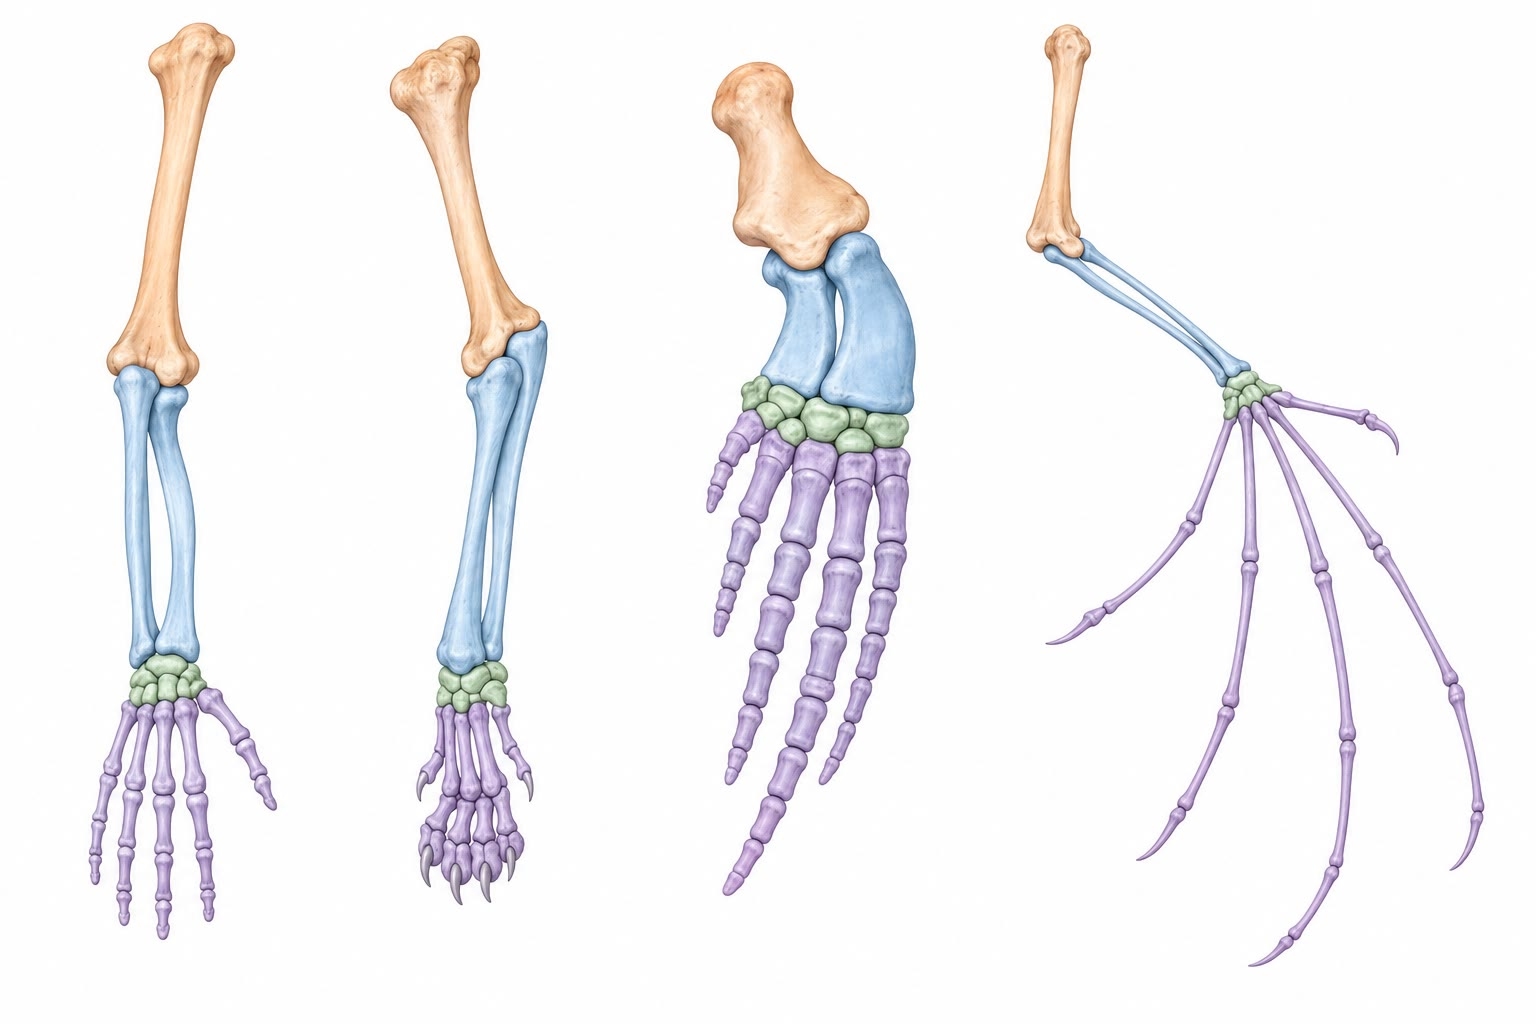
\includegraphics[width=0.66\linewidth]{images/book4/ai/b4-11-tetrapod-limbs.jpg}

{\small 同一方案、四种肢体：人、猫、
鲸和蝙蝠的前肢共享相同的骨骼，且排列顺序相同——
一块近端长骨、两根中段骨、腕部，以及指（趾），
由相同的信号中心构建，只在生长方式上有所不同。}
\end{omfigure}

\section{协调与雕塑}

\begin{proposition}[轴之间相互对话]\label{prop:b2:limb-organogenesis:loop}
\index{反馈环!发育性}
各中心相互维持：来自顶端嵴的 FGF 使 ZPA
持续表达 Shh，而 Shh 经中胚层中的一个中继，
使顶端嵴持续表达 FGF；去掉任一方，另一方会在一天内消退。
来自背侧外胚层的 Wnt7a 也是 Shh 充分表达所必需的，
并驱动中胚层的背侧命运（缺少它的小鼠有两个手掌）。这种
相互依赖构成一个
\emph{正反馈环}，将三个轴锁定在一起：
肢体只在被模式化的地方生长，也只在生长的地方被模式化，
因此芽不会长出没有前臂的手，
或类型错误的指（趾）。生长完成后，
环路被打破——中胚层停止中继，Shh 停止表达，
顶端嵴退化，肢体也就停止在其应有的大小。
\end{proposition}

\begin{proposition}[从模式到骨骼]\label{prop:b2:limb-organogenesis:skeleton}
\index{软骨发生}\index{细胞凋亡!趾间}
一旦被确定位置，离开生长区的中胚层细胞
\emph{凝结}成与未来骨骼形状相同的棒状和板状结构，
分化为分泌富含
胶原蛋白和蛋白聚糖基质的软骨细胞，并形成每一块
骨骼元件的软骨模型；关节形成于一带细胞被告知
不得分化为软骨之处；血管侵入这些模型，骨组织
由中心向外取代软骨，并在两端留下生长板，
使骨持续伸长直至成年
（\emph{软骨内成骨}）。来自\omterm{prop:b2:vertebrate-development:neurulation}{体节}的肌肉前体细胞
迁入其中、分裂，融合成肌纤维
（见\cref{ch:b2:cell-differentiation}），并通过肌腱附着，这些肌腱
由肢体自身的中胚层形成。指线之间的组织通过
程序性细胞死亡而被移除：趾间
蹼中的细胞受骨形态发生蛋白（BMP）信号的指示，启动
自身的死亡程序，并在一天内被清除，从而使
手指分开。鸭子保留趾蹼，是因为其
趾间组织表达一种 BMP 抑制剂；若把同样的抑制剂装在珠子上施于鸡，
则长出蹼足。
\end{proposition}
\begin{proof}[证据]
将鸡腿芽上切下的趾间中胚层移植到别处，
它按时死亡——死亡是内在的，在组织移除之前已被决定；
而取自鸭子的同样组织则存活。
将 BMP 珠子置于鸭子的趾间会使蹼死亡；
将抑制剂 gremlin 的珠子置于鸡的趾间，
则能保住蹼。肢体中缺少 BMP 受体的小鼠保留其趾蹼。
\end{proof}

\begin{omfigure}
\begin{tikzpicture}[every node/.style={font=\scriptsize}]
  \foreach \x/\lab in {0/{指（趾）列凝集 \\成软骨}, 4.2/{指（趾）间细胞 \\死亡（BMP）}, 8.4/{指（趾）分开；\\硬骨取代软骨}} {
    \begin{scope}[xshift=\x cm]
      \node[below, align=center] at (1.5,-0.3) {\lab};
    \end{scope}
  }
  % stage 1: paddle with rays
  \draw[thick, fill=omDef!8] (0,0) .. controls (0,2.2) and (3,2.2) .. (3,0) -- cycle;
  \foreach \x in {0.6,1.2,1.8,2.4} \draw[thick, fill=omDef!30, rounded corners=2pt] (\x-0.12,0.1) rectangle (\x+0.12,1.5);
  % stage 2: paddle with dying webs
  \begin{scope}[xshift=4.2cm]
    \draw[thick, fill=omDef!8] (0,0) .. controls (0,2.2) and (3,2.2) .. (3,0) -- cycle;
    \foreach \x in {0.6,1.2,1.8,2.4} \draw[thick, fill=omDef!30, rounded corners=2pt] (\x-0.12,0.1) rectangle (\x+0.12,1.5);
    \foreach \x in {0.9,1.5,2.1} \foreach \y in {0.7,1.0,1.3} \fill[omThm] (\x,\y) circle (0.05);
  \end{scope}
  % stage 3: separated digits
  \begin{scope}[xshift=8.4cm]
    \draw[thick, fill=omDef!8] (0,0) -- (0,0.5) -- (0.3,0.5) -- (0.35,1.7) -- (0.85,1.7) -- (0.9,0.5) -- (1.05,0.5) -- (1.1,1.85) -- (1.6,1.85) -- (1.65,0.5) -- (1.8,0.5) -- (1.85,1.7) -- (2.35,1.7) -- (2.4,0.5) -- (2.7,0.5) -- (2.7,0) -- cycle;
    \foreach \x in {0.6,1.35,2.1} \draw[thick, fill=omExo!60, rounded corners=2pt] (\x-0.1,0.1) rectangle (\x+0.1,1.4);
  \end{scope}
\end{tikzpicture}

{\small 雕塑手部：软骨指线在肢板中凝结，
其间的细胞死亡（红色），游离的手指骨化。}
\end{omfigure}

\begin{example}[同一肢体，生长各异]\label{ex:b2:limb-organogenesis:evolution}
蝙蝠的翼是一只手，其第 2 至第 5 指的长度
是小鼠的数倍——将一段肢体基因的增强子从蝙蝠移植到小鼠中，
会使小鼠前肢骨变长——而其趾间组织得以保留，
是因为趾蹼表达鸭子所用的
BMP 抑制剂。鲸的鳍是一只带有额外指骨的手，
趾间不发生死亡。马的腿是
单指结构，其余指已退化为细骨。蛇没有肢体，
是因为其体侧从不表达启动
芽形成的信号。鱼的鳍没有自足部，但由相同的 AER 和 ZPA 构建，
却在形成手指的晚期阶段之前即停止其 Hox 程序；
化石\emph{Tiktaalik}（3.75 亿年前）
表明腕部已出现在鳍中。肢体演化主要是
对一个保守程序的调节——每个阶段持续多久、
每种信号作用多远、哪些细胞死亡。
\end{example}

\section{练习}

\begin{exercise}[$\star$]\label{exo:b2:limb-organogenesis:1}
指出\omterm{def:b2:limb-organogenesis:bud}{肢芽}的三个轴，并对每个轴说明
其信号中心、位置及信号。
\end{exercise}

\begin{exercise}[$\star$]\label{exo:b2:limb-organogenesis:2}
给出肢体骨骼的三段，以及每段在人类手臂和腿中所含的骨。
哪些 Hox 基因标记了它们？
\end{exercise}

\begin{exercise}[$\star$]\label{exo:b2:limb-organogenesis:3}
按顺序列出从一小片侧板中胚层
发育为带有骨、关节和肌肉的手指的各步骤。
\end{exercise}

\begin{exercise}[$\star$]\label{exo:b2:limb-organogenesis:4}
若 AER 被去除，肢体会呈何种形态：(a) 一旦
芽出现即去除，(b) 前臂确定之后去除，(c) 不去除，
而代之以一颗 FGF 珠？
\end{exercise}

\begin{exercise}[$\star\star$]\label{exo:b2:limb-organogenesis:5}
设 $\lambda = \qty{40}{\micro m}$，第 4、3、2 指的阈值分别为源浓度的 $0.5$、$0.2$
和 $0.05$，计算
三条边界及各指区的宽度。
\end{exercise}

\begin{exercise}[$\star\star$]\label{exo:b2:limb-organogenesis:6}
预测以下处理后鸡翅的指型：(a) 完整的 ZPA
移植到前缘；(b) 移植四分之一数量的
ZPA 细胞；(c) 前缘的一颗 Shh 珠经短时间
作用后移除。试从剂量与时间两方面分别解释。
\end{exercise}

\begin{exercise}[$\star\star$]\label{exo:b2:limb-organogenesis:7}
鸡的\omterm{def:b2:limb-organogenesis:bud}{肢芽}在嵴形成时有 \num{5000} 个细胞，
其细胞每 \qty{12}{h} 分裂一次。四天后有多少细胞？若
该阶段肢体有 $4\times 10^{6}$ 个细胞，则细胞周期
或细胞死亡须满足什么条件？
\end{exercise}

\begin{exercise}[$\star\star$]\label{exo:b2:limb-organogenesis:8}
解释为何鸡具有分离的趾而鸭具有蹼状足，以及
在鸡胚趾间放置一颗 BMP 抑制剂珠会产生何种效应。
指间细胞死亡的内在时序（在移植物中按时发生）说明了
细胞是如何被指令的？
\end{exercise}

\begin{exercise}[$\star\star$]\label{exo:b2:limb-organogenesis:9}
一只小鼠缺失 Hoxa13 和 Hoxd13，另一只缺失 Hoxa11 和
Hoxd11。预测每只前肢的骨骼，并说明该结果
表明 Hox 结构域与节段之间有何联系。
\end{exercise}

\begin{exercise}[$\star\star\star$]\label{exo:b2:limb-organogenesis:10}
解释 AER 与 ZPA 之间的正反馈，以及它为何
使肢体稳健，并说明若 Shh 不能维持 FGF，芽会
发生什么。将其与
\cref{ch:b2:mammal-reproduction}中分娩的正反馈相比较：各循环由什么终止？
\end{exercise}

\begin{exercise}[$\star\star\star$]\label{exo:b2:limb-organogenesis:11}
蝙蝠的第三指相对于体型，比小鼠的
长八倍。若指软骨在生长窗口期内以指数方式
按每天 $r$ 的速率延长，且蝙蝠的窗口期比小鼠
长四天，则需要多大的 $r$？给出两种发育变化
（一种在生长中，一种在细胞死亡中），使
手转变为翼。
\end{exercise}

\begin{exercise}[$\star\star\star$]\label{exo:b2:limb-organogenesis:12}
Sonic hedgehog 自底板起对\omterm{prop:b2:vertebrate-development:neurulation}{神经管}进行模式化
（见\cref{ch:b2:vertebrate-development}），并自 ZPA 对指进行模式化。
试讨论为何演化会将少数信号用于多种功能，以及同一分子
在不同组织中如何具有不同含义，并
说明这对此类基因\omterm{def:b2:genome-diversification:mutation}{突变}的效应意味着什么。
\end{exercise}

\section{问题：一周内建成的翼}

\begin{problem}[{周末问题——追踪鸡翼自芽到骨骼的过程：
其分裂生长、桑德斯嵴切除实验的时间安排，
Shh 梯度的计算及其重复的预测、蹼
的塑形、翼与蝙蝠翼的比较，最终归结为倍增
次数、指的边界，以及镜像重复所需芽的
宽度}]
\label{pb:b2:limb-organogenesis:1}
鸡翼芽在孵化第 3 天出现，含 \num{2000} 个
中胚层细胞，长度为 \qty{0.4}{mm}；至第 7 天时翼
长 \qty{4}{mm}，其体积为芽的 \num{1000} 倍。\omterm{prop:b2:limb-organogenesis:aer}{进展
区}细胞每 \qty{12}{h} 分裂一次。嵴切除：第 3.0 天时
肢体为残端；第 3.5 天时仅余肱骨；第 4.0 天时为肱骨、
桡骨和尺骨；第 4.5 天时为仅缺指尖的翼。
Shh：$D = \qty{1e-12}{m^2/s}$，半衰期 \qty{29}{min}；阈值
分别为 $0.6$、$0.25$、$0.08$ 乘 $c_0$（第 4、3、2 指），芽宽（由后
至前）\qty{600}{\micro m}。指间蹼：三个区域
各为 \qty{300}{\micro m}$\times$\qty{300}{\micro m}$\times$\qty{200}{\micro m}，细胞
体积为 \qty{1000}{\micro m^3}，在 \qty{24}{h} 内被清除。

\medskip
\noindent\textbf{第一部分——生长。}
\begin{enumerate}
  \item 四天内发生多少次倍增？由 \num{2000} 个细胞
        出发，可得多少个细胞？
  \item 与千倍的体积增长相比较：细胞增大与基质
        须共同提供多大的倍数？
  \item 长度增加了多少倍？若芽以恒定半径的圆柱体方式
        生长，则体积增加的倍数为多少，
        此差异说明了关于形状的什么？
  \item 嵴的 FGF 可深入中胚层 \qty{300}{\micro m}。
        在第 3 天和第 7 天时，芽受其影响的
        部分占多大比例？
  \item 解释为何在生长的器官中，作用距离固定的信号
        会产生近–远轴序列。
  \item 一个细胞在第 4 天离开\omterm{prop:b2:limb-organogenesis:aer}{进展区}，
        它将并入哪一节段？
\end{enumerate}

\medskip
\noindent\textbf{第二部分——节段的时序。}
\begin{enumerate}[resume]
  \item 由切除系列，给出每一节段
        （近段柱节、中段轭节、远段自节）被确定的时间。
  \item 相继确定的节段之间，相隔多少个
        细胞周期？
  \item 从\omterm{prop:b2:limb-organogenesis:aer}{进展区}和
        Hox 结构域的角度解释该结果。
  \item 在嵴于第 3.5
        天被切除的芽上放置一颗 FGF 珠，预测该肢体。
  \item 将第二个嵴移植到一个
        第 3.5 天的完整芽的背侧表面，预测其结果。
  \item 芽为何在第 7 天停止生长，
        而非无限期地持续生长？
\end{enumerate}

\medskip
\noindent\textbf{第三部分——梯度。}
\begin{enumerate}[resume]
  \item 计算 Shh 的 $k$ 和 $\lambda$。
  \item 计算三个指（趾）边界及其区域宽度。
  \item 在一个不形成指（趾）的前部区域，
        芽宽 \qty{600}{\micro m} 时，该区域有多宽？
  \item 一次\omterm{def:b2:genome-diversification:mutation}{突变}使 Shh 的输出量加倍。重新计算边界，
        并判断是否形成额外的指（趾），以及是哪一个。
  \item 将 ZPA 移植到前缘。芽的最小宽度须为多少，
        才能形成完整的镜像组 4-3-2-2-3-4，而两个 2 号指（趾）区域不重叠？
        鸡芽的宽度是否
        足够？
  \item 若芽的宽度仅为 \qty{200}{\micro m}，
        则预测其模式。
  \item 为何移植四分之一的 ZPA 只得到 2-2-3-4？
\end{enumerate}

\medskip
\noindent\textbf{第四部分——雕塑与演化。}
\begin{enumerate}[resume]
  \item 计算三张蹼中的细胞数，以及清除期间的细胞死亡速率，
        以每秒细胞数计。
  \item 鸭的指间细胞表达一种 BMP 抑制剂。预测
        在鸭蹼中加入一颗 BMP 珠的效应，以及在鸡蹼中
        该抑制剂的效应。
  \item 蝙蝠的指（趾）软骨再额外生长四天，
        以指数速率 \qty{0.5}{d^{-1}} 生长。它比鸡的
        软骨长多少倍？另说出使翼膜得以形成的
        第二项变化。
  \item 一个鱼鳍芽具有 AER 和 ZPA，但没有指（趾）。缺少的是什么，
        以及 \emph{Tiktaalik} 表明了什么？
  \item 若蹼细胞改由分裂产生，
        从 \num{1000} 个奠基细胞出发，每个周期 \qty{12}{h}，则产生它们需要多长时间？
        将其与清除它们所需的
        一天相比较。
  \item 给出结果：四天内的倍增次数、三个指（趾）边界，
        以及镜像重复所需的最小宽度。
\end{enumerate}
\end{problem}
